\documentclass[upright, contnum]{umemoria}
\depto{DEPARTAMENTO DE CIENCIAS DE LA COMPUTACIÓN}
\author{NICOLÁS SALAS VEGA}
\title{DESARROLLO DE UN SISTEMA DE EVALUACIÓN DE POSTULACIONES AL MAGÍSTER EN TECNOLOGÍAS DE LA INFORMACIÓN}
\auspicio{.}
\date{ABRIL 2021}
\guia{SERGIO OCHOA, DANIEL PEROVICH}
\carrera{INGENIERO CIVIL EN COMPUTACIÓN}
\memoria{MEMORIA PARA OPTAR AL TÍTULO DE}
\comision{JUAN ÁLVAREZ, CLAUDIO GUTIÉRREZ}

% Prevenir quiebre de palabras
\tolerance=1
\emergencystretch=\maxdimen
\hyphenpenalty=10000
\hbadness=10000

\usepackage{lipsum}

% \usepackage[latin1]{inputenc}
% \usepackage[T1]{fontenc}

\begin{document}

\frontmatter
\maketitle

\begin{abstract}
    El Programa de Magíster en Tecnologías de la Información (MTI), que imparte
    el Departamento de Ciencias de la Computación de la Universidad de Chile,
    recibe de forma \emph{online} postulaciones de ingreso al programa a través
    de la plataforma UCampus. Estas postulaciones deben ser descargadas por el
    personal de apoyo, y luego evaluadas por miembros del comité académico del
    programa. Estos últimos emiten una recomendación de aceptación o rechazo
    para cada postulación. El coordinador del programa analiza esas
    recomendaciones y emite una resolución al respecto.

    Actualmente, el proceso de evaluación de cada postulación se lleva a cabo a
    través del intercambio de correos electrónicos, coordinados en gran medida
    por el personal de apoyo al programa. Estas personas se encargan de enviar
    los antecedentes a los evaluadores, y solicitar su recomendación de
    aceptación o rechazo, recolectar las recomendaciones, y enviárselas al
    coordinador para que emita una resolución. Todo esto, con las limitaciones
    típicas del intercambio de correos electrónicos en términos de eficiencia
    del procesamiento y la eventual pérdida de información.
    
    Por otra parte, esta forma de procesar las evaluaciones no permite extraer
    estadísticas o mantener la historia de las evaluaciones. Sin datos
    fidedignos acerca del funcionamiento de este proceso, se vuelve difícil
    poder mejorarlo. Hoy en día el MTI representa un canal importante de
    transferencia de conocimiento desde el Departamento hacia la industria, por
    lo tanto, todos sus procesos deben funcionar lo mejor posible.
    
    El objetivo de este trabajo de memoria es desarrollar un sistema que permita
    automatizar gran parte del procesamiento de las postulaciones al MTI,
    alivianando la carga de trabajo sobre las personas involucradas, mejorando
    la gestión de éste, y la capacidad de medir distintos aspectos del proceso.
    
    Para alcanzar el objetivo planteado se desarrolló un sistema web que
    gestiona las evaluaciones de las postulaciones. Éste extrae los datos desde
    UCampus utilizando un scraper, almacena las postulaciones en su base de
    datos, e implementa un workflow que automatiza gran parte del proceso antes
    descrito.
    
    Debido al esfuerzo que requiere la ejecución de dicho workflow, así como el
    número de participantes que intervienen en él, la solución desarrollada fue
    evaluada con postulaciones de prueba (con información ficticia), donde dos
    miembros del comité académico ejecutaron el proceso completo. Durante las
    pruebas, estas personas debieron asumir los distintos roles involucrados en
    el proceso, y tomar las acciones correspondientes a dichos roles.
    
    Como resultado de las pruebas se vió que el sistema soporta correctamente el
    proceso de evaluación de postulaciones, y sólo se indicaron mejoras a la
    usabilidad de las interfaces del mismo. Estas mejoras serán abordadas como
    parte del trabajo a futuro de este proyecto.
    
\end{abstract}

\begin{dedicatoria}
Una dedicatoria corta.
\end{dedicatoria}

\begin{thanks}
\lipsum[1-2]
\end{thanks}

\cleardoublepage
\tableofcontents
\cleardoublepage
\listoftables
\cleardoublepage
\listoffigures

\mainmatter

\begin{intro}
	El Departamento de Ciencias de la Computación de la Universidad de Chile
	ofrece distintos programas de magíster. Uno de ellos es el Magíster en
	Tecnologías de la Información (en adelante MTI). Uno de los objetivos de
	este programa es formar especialistas con conocimientos de aspectos
	aplicados respecto al uso, gestión y adopción de Tecnologías de la
	Información y Comunicaciones.

	Teniendo en cuenta el perfil de los profesionales que busca formar este
	programa, y la naturaleza misma del magíster, resulta razonable pensar que
	el proceso de postulación al mismo, así como el procesamiento de dichas
	postulaciones, se haga usando herramientas computacionales.
	
	Hoy en día, la postulación a este programa se hace a través de la plataforma
	UCampus\footnote{UCampus es un Centro Tecnológico que desarrolla plataformas
	de apoyo a la gestión, automatizando los procesos de Instituciones de
	Educación Superior, en particular el de la Universidad de Chile.
	https://ucampus.cl.}. En esa plataforma, el postulante debe ingresar sus
	datos personales, y adjuntar un conjunto de documentos relevantes para
	respaldar su  postulación. Entre esos documentos están las cartas de
	recomendación, el currículum del postulante, su certificado de título y su
	carta motivacional.
	
	Una vez enviada la postulación a través de UCampus, los documentos quedan
	disponibles para que cada programa (en este caso, el MTI) haga con ellos lo
	que estime conveniente. UCampus no ofrece la funcionalidad para apoyar el
	procesamiento de las postulaciones, por lo que cada programa debe hacerlo
	por fuera de esta plataforma. 

	\section{Problema Abordado}

	El proceso de evaluación de postulaciones al MTI se realiza en forma manual.
	Para ello, un funcionario del Programa de Educación Continua (PEC) del DCC
	inicia el proceso descargando manualmente cada uno de los archivos subidos a
	UCampus por el postulante. Esa información luego es enviada a los miembros
	del comité académico del programa a través de un correo electrónico. Los
	miembros de ese comité evalúan las postulaciones. Estas personas pueden
	solicitar información adicional al postulante en caso que se requiera; y en
	esos casos, el funcionario del PEC actúa como intermediario entre el
	postulante y el comité académico.

	Cuando la información de una postulación está completa, los evaluadores emiten
	un juicio individual y justificado respecto a la admisión o no de cada
	postulante al programa. Esta información es enviada vía correo electrónico al
	funcionario del PEC, quien reúne todas las opiniones de los evaluadores acerca
	de una postulación, y luego se las envía al coordinador del programa para que
	decida la admisión o rechazo del postulante. En esa instancia, el coordinador
	revisa manualmente todas las evaluaciones y emite un juicio formal, el cual debe
	ser registrado en la plataforma UCampus, e informado al postulante.

	Este flujo de trabajo (workflow) es completamente informal, por lo que los
	tiempos de procesamiento de una postulación varían mucho, dependiendo de la
	carga de trabajo que tengan los funcionarios del PEC y el resto de los
	participantes. Dado que hoy en día las evaluaciones de las postulaciones se
	realizan de forma manual, el proceso se vuelve lento, costoso y propenso a
	errores. Además, el flujo de trabajo asociado a este proceso es muy difícil de
	monitorear, medir y mejorar. Otro aspecto importante es que este proceso manual
	no escala bien, por lo que se requieren sistemas de apoyo al procesamiento de
	estas postulaciones.

	Tomando en cuenta lo anterior, en esta memoria se diseñó e implementó un sistema Web que:

	\begin{enumerate}
		\item Agiliza el proceso de evaluación de postulaciones al MTI.
		\item Facilita la recopilación y almacenamiento de datos relevantes,
		tanto del postulante como de la evaluación de su postulación.
	\end{enumerate}

	El sistema no busca extender la funcionalidad de UCampus, ni la validez de
	la postulación, por lo tanto, en la memoria se asume que los datos que
	provienen de dicha plataforma son correctos. 

	\section{Objetivos de la Memoria}

	El objetivo general de esta memoria fue desarrollar un sistema Web que
	automatiza parte del flujo de trabajo asociado al procesamiento de
	postulaciones al Magíster en Tecnologías de la Información; programa que es
	impartido por la Escuela de Postgrado de la FCFM\footnote{Facultad de
	Ciencias Físicas y Matemáticas de la Universidad de Chile} a través del
	DCC\footnote{Departamento de Ciencias de la Computación}. Los objetivos
	específicos definidos para alcanzar el objetivo general fueron los
	siguientes:

	\begin{enumerate}
		\item Desarrollar un servicio de software que extraiga automáticamente
		la información de las postulaciones al programa, desde la plataforma
		UCampus.
		\item Desarrollar un sistema que automatice el flujo de trabajo
		(workflow) de evaluación de las postulaciones.
		\item Desarrollar un servicio que facilite la toma de decisiones del
		Coordinador del Programa, respecto a la aceptación o rechazo de los
		postulantes, y a la comunicación de éste con la Escuela de Postgrado.
	\end{enumerate}


	\section{Estructura del Documento}
	**Falta añadir aquí la estructura del documento**.
\end{intro}
\chapter{Análisis del escenario legado}

A continuación se indican los roles de los participantes en el proceso de
evaluación de postulaciones. Luego se describe y discute dicho proceso.
Finalmente, se analizan las alternativas para extraer la información de las
postulaciones desde UCampus, y de esa manera poder alimentar el sistema
desarrollado en esta memoria.

\section{Participantes en el Proceso de Evaluación de Postulaciones}

% Wrappear la tabla...
\begin{table}[ht]
    \begin{center}
        \begin{tabular}{|l|l|}
            \hline \\
            Rol & Descripción \\ \hline

            Postulante & Genera una postulación a través de UCampus. Una vez
            entregada la postulación completa, éste espera por el resultado
            (aceptación o rechazo) de la misma.\\ \hline

            Miembro del Comité Académico del Programa & Evalúa las
            postulaciones, emite un voto y entrega su opinión al Coordinador de
            Magíster en forma de comentarios. Estos comentarios justifican la
            opinión del miembro correspondiente respecto a la aceptación o
            rechazo de un postulante \\ \hline

            Coordinador de Magíster / Presidente del Comité Académico & Resuelve
            una postulación. La decisión es tomada en base a las evaluaciones
            realizadas por los miembros del comité. \\ \hline

            Asistente / Funcionario del PEC & Se encarga de revisar la validez
            de los documentos adjuntados a la postulación, y deriva la
            información al Coordinador del Magíster y a los miembros del Comité
            Académico del Programa cuando corresponde. Los asistentes
            (funcionarios) son quienes llevan a cabo la mayor parte del workflow
            manual involucrado en el procesamiento de las postulaciones. \\ \hline
        \end{tabular}
    \end{center}
\end{table}


\section{Proceso a apoyar}

Tomando en cuenta el rol de cada actor, a continuación se resume el proceso que
sigue una postulación hasta lograr un veredicto de aceptación o rechazo.

% Figura
\begin{figure}[!ht]
    \begin{center}
        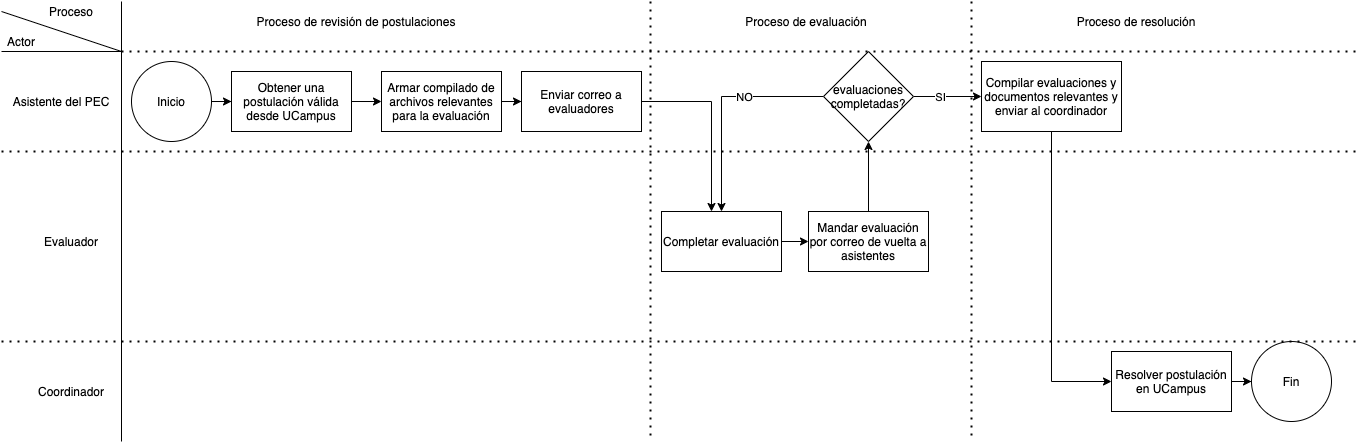
\includegraphics[scale=0.3]{imagenes/01-workflow-legado.png}
    \end{center}
    \caption{Workflow del proceso de evaluación de postulaciones}
    \label{workflow-legado}
\end{figure}

Tal como se puede ver en la figura \ref{workflow-legado}, el proceso involucra
los siguientes 7 pasos:

\begin{enumerate}
    \item Un postulante ingresa una postulación a través de UCampus.
    \item Los asistentes revisan la validez y completitud de la postulación. En
    caso de ser válida y estar completa, la información asociada a ésta se envía
    al Coordinador del Programa y a los Miembros del Comité Académico vía correo
    electrónico.
    \item El Coordinador del Programa y los Miembros del Comité Académico
    evalúan cada postulación, y emiten un juicio individual acerca de la
    aceptación o rechazo del postulante al programa, teniendo en cuenta las
    exigencias establecidas en la normativa vigente del MTI.
    \item Cada evaluador envía por correo sus evaluaciones al asistente, quien
    las recolecta y envía al Coordinador del Programa el conjunto de todas las
    evaluaciones recibidas.
    \item El Coordinador del Programa revisa todas las opiniones de los
    evaluadores y emite un veredicto acerca de la aceptación o rechazo del
    postulante.
    \item El Coordinador del Programa registra la decisión en UCampus y entrega
    a los asistentes un formulario de resolución firmado.
    \item Los asistentes envían el formulario a la Escuela de Postgrado, quien
    notifica al postulante.
\end{enumerate}

En el paso 2, la postulación puede ser devuelta al postulante para que corrija
errores en caso de que existan, o para que éste envíe los documentos faltantes.
Después de una revisión del proceso con el coordinador del programa y miembros
del comité académico, se determinó que el diseño del mismo era apropiado. Las
falencias del mismo radican principalmente en la artesanalidad e informalidad
con la que se realizan las actividades que son parte del mismo. Por lo tanto, la
automatización de algunas de esas actividades parece ser suficiente para mejorar
considerablemente la calidad y predictibilidad del proceso en términos de su
duración.

\section{Obtención de Datos desde la Plataforma UCampus}

Respecto de la obtención de datos de las postulaciones (desde UCampus), a pesar
de que exista una API publicada por su equipo desarrollador, ésta no incluye
end-points que permiten obtener los datos de las postulaciones al magíster, lo
cual va en contra del primer propósito: “permitir agilizar el proceso de
postulaciones”. 

Para resolver este problema, una solución que no involucra trabajo extra de los
usuarios es hacer \emph{scraping} de la página de postulaciones de UCampus. En
ella se muestra una tabla con todas las postulaciones y un link de detalle a
cada una de ellas, desde donde se puede obtener la información de todas las
postulaciones al programa. Teniendo esta información, ya sea vía scraping o via
una extensión a la API de UCampus, es posible construir un proceso autónomo que
recupere la información de las postulaciones, sin que se requiera coordinación
manual del proceso por parte de los Asistentes o del Coordinador del Programa.

Para agilizar el procesamiento de las postulaciones, el sistema enviará avisos a
los usuarios relevantes cuando se requiere que tomen alguna acción, evitando así
que estos tengan que estar pendientes de ingresar al sistema para ver si tienen
alguna asignación sobre la cual responder. Un estudio realizado por la empresa
Microsoft constató que este envío de avisos concientiza a las personas de que
hay cosas pendientes, y aunque distrae, es preferido por su valor en la
concientización [1].

Con respecto a la facilidad de recopilación y almacenamiento de los datos
relevantes de los postulantes, usar una base de datos para dicho propósito es
mejor que mantener los datos en las cuentas de correo de los participantes en el
proceso. Si bien algunos datos están disponibles en UCampus (como los resultados
de las postulaciones, por ejemplo), las opiniones de los Miembros del Comité
Académico, entre otros datos, quedan en la cadena de correos asociada a una
publicación. Usando una base de datos, estos datos serán luego fáciles de
acceder, por ejemplo, para realizar un análisis de la efectividad y eficiencia
del procesamiento de las postulaciones.

El desarrollo de este sistema cuenta con los siguientes desafíos:

\begin{enumerate}
    \item UCampus no entrega información estructurada respecto a postulaciones
    al magíster, y se pretende que la alimentación de datos sea realizada de
    forma automática.
    \item El sistema debe automatizar el flujo de trabajo, invitando a los
    participantes (roles involucrados en el proceso) a completar sus tareas lo
    más rápido posible, manteniéndolos informados acerca de tareas que
    eventualmente ellos tengan pendientes de realizar.
    \item El sistema debe garantizar que cada actor del proceso pueda hacer sólo
    lo que su rol permite, y nada más.
\end{enumerate}


\section{Análisis de Alternativas de Interacción con UCampus}

En esta sección se describen las tareas realizadas en la búsqueda de una
solución a la extracción automática de información desde UCampus. En particular
se indican los desafíos asociados a los problemas que hay que resolver, las
alternativas para abordarlos y las propuestas de solución.

\subsection{Posible Extensión de la API de UCampus}

Una de las primeras tareas realizadas fue comunicarse con el área de desarrollo
de UCampus, para explorar la factibilidad de implementar un nuevo endpoint en su
API, con el objetivo de permitir la extracción de los datos de las postulaciones
desde una aplicación externa; en este caso, nuestro sistema de evaluación. Si
bien la respuesta fue pronta y con buena disposición, no se dió curso a la
solicitud por las siguientes razones:

\begin{itemize}
    \item El formulario de ingreso de datos y el flujo de una postulación están en
    el sistema llamado ``Workflow'', el cual está a cargo del ADI (Área de
    Infotecnologías), y por lo tanto, poco puede ayudar el Centro UCampus a la
    intervención de dicho sistema. Además, no hay una conexión directa entre el
    sistema de ADI y la plataforma UCampus, por lo que se requiere realizar bastante
    trabajo para poder contar con información de postulaciones a través de la API de
    UCampus.
    \item La respuesta desde ADI fue que los datos se encuentran encapsulados dentro
    de herramientas internas del sistema ``Workflow'', lo cual dificulta la extracción
    de datos limpios desde su base de datos.
\end{itemize}

En resumen, y aunque aún no está completamente cerrada la posibilidad de obtener
los datos desde la fuente, se hace necesario explorar otras opciones, las cuales
se detallan a continuación.

\subsection{Extracción de Datos de UCampus Usando Scrapers}

Scraping es una técnica que se usa para la extracción de datos no estructurados,
ya sea a partir de imágenes, PDFs, o páginas web, entre otros. Al no poder
obtener directamente los datos de postulaciones a través de una API (o una
interfaz de acceso a datos similar), usar un scraper es una buena alternativa
para recuperar dicha información. En este caso, los datos de las postulaciones
se encuentran accesibles a través de una interfaz Web de la plataforma UCampus,
siempre que se cuente con los derechos para ello. Este es el canal oficial tanto
para postular, como para gestionar las postulaciones.

El uso de scrapers no está exento de desafíos. Algunos de los más conocidos son
los siguientes: 

\begin{itemize}
    \item Si el sitio web que representa la fuente de datos cambia su interfaz
    de usuario, entonces se debe adaptar el scraper para extraer información del
    nuevo layout de la página.
    \item Algunos sitios web (y este es el caso de UCampus) usan Javascript en
    su interfaz (versiones modernas). Esto hace que no sea trivial la extracción
    de los datos, pues el scraper debe esperar por eventos asíncronos para poder
    extraer datos. Las librerías tradicionales de scraping [6, 7] no cuentan con
    esa capacidad.
\end{itemize}

A pesar de lo planteado anteriormente, usar un scraper es realmente la única
alternativa que existe hoy para poder extraer los datos de las postulaciones de
forma automática. Con respecto a las alternativas para hacer el scraping, se
analizaron las siguientes librerías, dado que están dentro de las más
reconocidas:

\begin{itemize}
    \item \emph{Puppeteer} [3]: Librería Node.js que permite controlar una instancia de
    Chrome a través del protocolo DevTools.
    \item \emph{Selenium WebDriver} [4]: Esta es una API con implementación en
    múltiples lenguajes, orientada al testing, que permite manejar un browser.
\end{itemize}

Las diferencias entre estas librerías radica principalmente en que Puppeteer
controla instancias de Chrome, mientras que Selenium es una implementación para
un navegador genérico. Ambas cumplen el propósito de extraer datos desde UCampus
sin problemas [8]. En el repositorio referenciado se muestran los resultados de
extraer ciertos datos desde UCampus con la cuenta del autor, de acuerdo a la
siguiente secuencia de pasos:

\begin{enumerate}
    \item Ingresar a UCampus con usuario y contraseña.
    \item Hacer clic en la pestaña Tareas Iniciadas.
    \item Extraer links desde una tabla. Cada caso particular (postulación)
    corresponde a una “Solicitud de Inscripción con Excepción (SIEs)”.
    \item Visitar todos los links disponibles y extraer sus datos.
\end{enumerate}

Con el objetivo de mantener la estabilidad del scraper, en el sentido de que
éste soporte la mayor cantidad de alternativas posibles para abordar los
eventuales cambios en la interfaz de usuario, puppeteer es la mejor opción. El
hecho de que la librería esté construida sobre Chromium hace que se pueda usar
todo el abanico de herramientas de Chrome para obtener datos, y manipular el
sitio web. Otro argumento para lo mismo es la frecuencia de actualizaciones. Los
drivers de Selenium mantienen su última fecha de liberación (para Python) el 1
de noviembre de 2018, mientras que Puppeteer lanzó su última versión el 26 de
febrero de 2021.

Debido a esto, y tomando en cuenta la cantidad de postulantes al MTI, resulta
válido también explorar la posibilidad de que los datos sean ingresados
manualmente al sistema por parte de sus usuarios; particularmente, por los
funcionarios del PEC.

\subsection{Carga Manual de datos de Postulaciones}

Si bien lo ideal es que los datos sean ingresados de forma automática al
sistema, no hay que perder de vista que el objetivo principal de este trabajo
es: \emph{desarrollar un sistema Web que automatice el flujo de trabajo asociado
al procesamiento de postulaciones al Magíster en Tecnologías de la Información}.
Con eso en cuenta, la carga manual de datos se percibe más bien como un
despropósito en este escenario.

Por otra parte, los scrapers anteriormente descritos fueron probados con
resultados satisfactorios que, en una primera aproximación, demostraron que es
posible extraer datos no estructurados desde UCampus, y confiar en los
resultados de dicho proceso. 

\section{Formulario de Postulación al MTI}

A continuación se muestra un formulario típico de postulación al MTI,
implementado sobre la plataforma UCampus. Se han ofuscado los datos sensibles
del postulante.

\begin{figure}[!ht]
    \begin{center}
        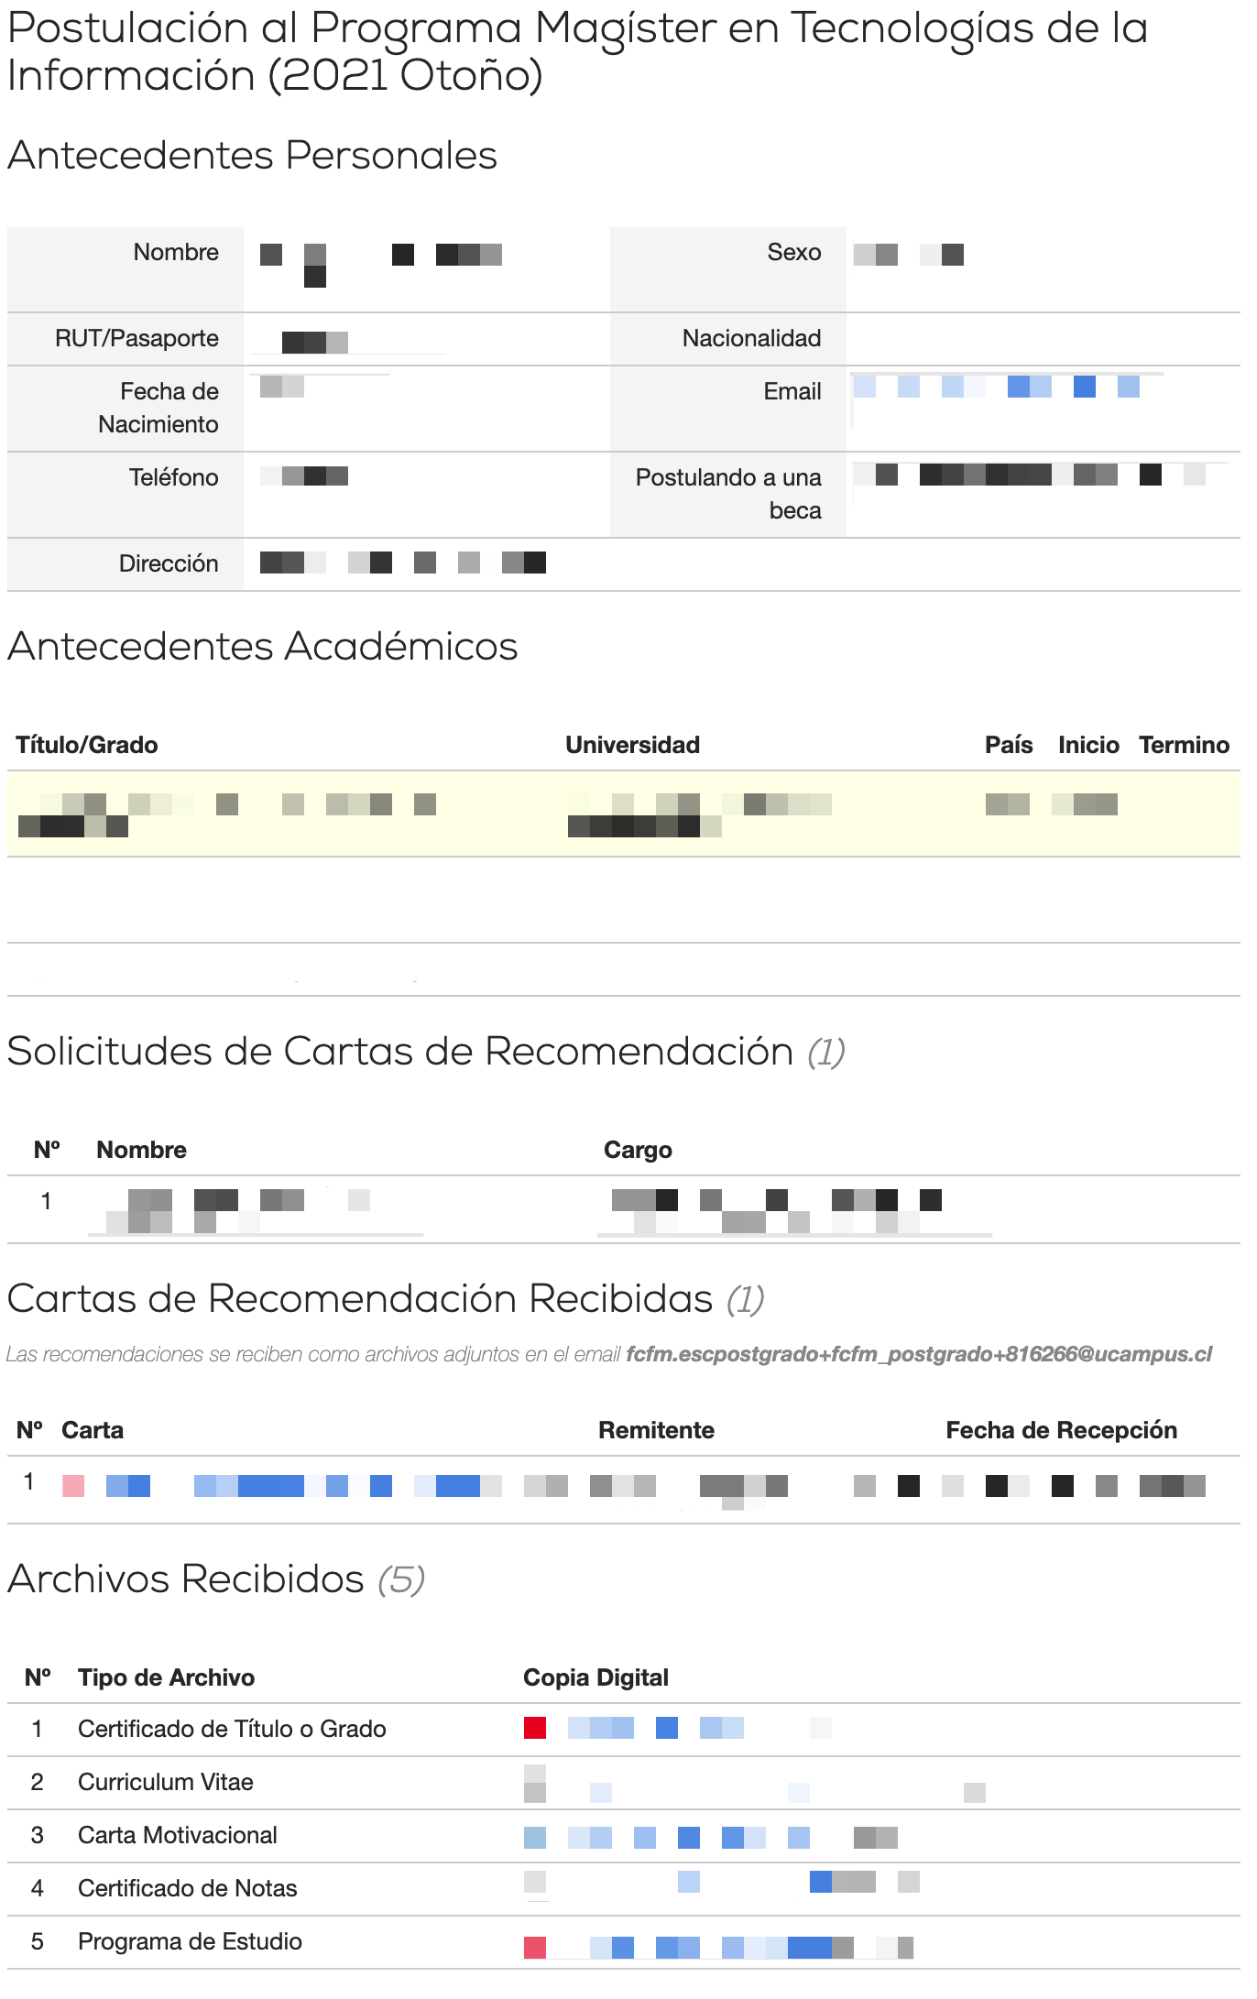
\includegraphics[scale=0.3]{imagenes/01-formulario-postulacion.png}
    \end{center}
    \caption{Formulario de postulación al Magíster en TI}
    \label{formulario-postulacion}
\end{figure}

Como se puede ver en la Figura \ref{formulario-postulacion}, una postulación
completa consta de los siguientes antecedentes:

\begin{itemize}
    \item Datos personales del alumno.
    \item Los antecedentes académicos del mismo: Título o grado, Universidad, País
    de la Universidad, Año de inicio y término de sus estudios.
    \item Solicitudes de cartas de recomendación, hechas por el postulante. Éstas se
    muestran por el nombre de cada persona a la que se le solicitó una carta de
    recomendación, su correo electrónico y su cargo.
    \item Cartas de recomendación recibidas. Éstas muestran el archivo
    correspondiente a la carta de recomendación, el nombre de la persona que lo
    envió, su email y la fecha de recepción.
    \item Los 5 archivos mandatorios de cada postulación: Certificado de título o
    grado, currículum vitae, carta motivacional, certificado de notas y el programa
    de estudio.
\end{itemize}

Algunas consideraciones a destacar del formato de los datos:

\begin{itemize}
    \item La fecha de nacimiento de un alumno sólo está presente para usuarios
    antiguos de UCampus. Usualmente ese campo sólo muestra la edad.
    \item La nacionalidad, de la misma forma, no suele estar presente en la
    postulación.
    \item La postulación puede estar a medio hacer. Vale decir, puede ser que la
    postulación no contenga las cartas de recomendación o documentos esenciales,
    y aún así el sistema permite que la misma sea enviada al coordinador del
    programa.
\end{itemize}
\chapter{Segundo}
\lipsum[50-60]
\begin{conclusion}
	\lipsum[130-132]
	\begin{figure}[!h]
		\centering
		
\includegraphics[scale=.2]{imagenes/fcfm.pdf}
		\caption{Logo de la Facultad}
		\label{logofcfm}
	\end{figure}
	\lipsum[133-134]
	\begin{table}[!h]
		\centering
		\begin{tabular}{|c||c|}
			\hline
			Campo 1& Campo 2\\\hline
			Valor 1& Valor2\\\hline
		\end{tabular}
		\caption{Tabla 1}
		\label{tabla:1}
	\end{table}
	\lipsum[135]
\end{conclusion}


\nocite{*}
\bibliographystyle{plain}
\bibliography{bibliografia}
\end{document}
